\documentclass[11pt]{article}
\usepackage[top=30truemm,bottom=30truemm,left=25truemm,right=25truemm]{geometry}
\usepackage[dvipdfmx]{graphicx}
\begin{document}
\title{偏光板を使った楕円偏光解析}
\author{平松}
\maketitle

\begin{figure}[htbp]
\centering
  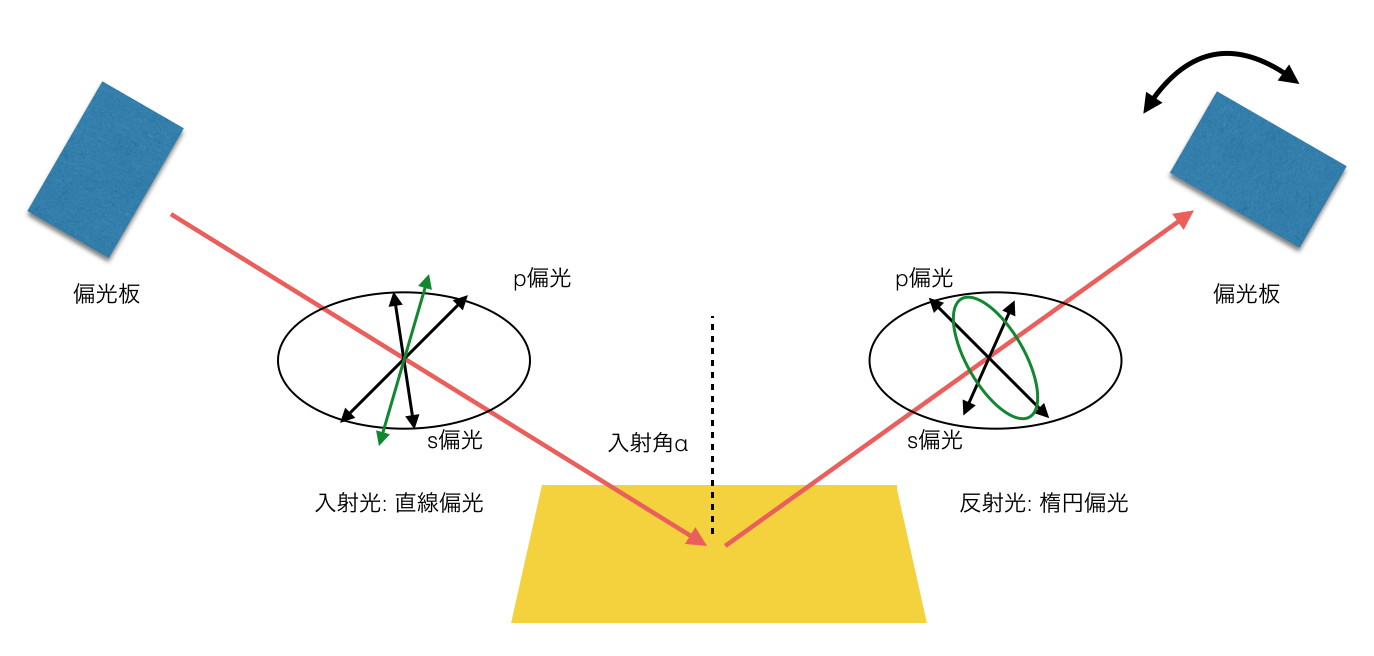
\includegraphics[width=13cm]{./schematics}
\end{figure}

反射光の楕円偏光解析を行い、誘電率を推定する。この際に反射光は完全偏光していると仮定しジョーンズ計算法を用い、ジョーンズベクトルの第1成分をs偏光、第2成分をp偏光に対応させる。\\

薄膜の等方性を仮定すると、反射によるs偏光からp偏光やp偏光からs偏光への散乱は無視できる。したがって入射光のジョーンズベクトルを$^t(E_s\ E_p)$、反射光のジョーンズベクトルを$^t(E'_s\ E'_p)$、s偏光とp偏光の複素反射率をそれぞれ$R_s, R_p$とすると、以下の関係がある。なお複素反射率には反射効率と位相の遅れの情報が含まれる。

\begin{eqnarray*}
  \left(
    \begin{array}{c}
      E'_s \\
      E'_p \\
    \end{array} 
  \right) 
  =
  \left(
    \begin{array}{cc}
      R_s & 0 \\
      0 & R_p \\
    \end{array}
  \right)
  \left(
    \begin{array}{c}
      E_s \\
      E_p \\
    \end{array}
  \right) \\
  \end{eqnarray*}
  
 入射光を直線偏光と仮定するとジョーンズベクトル$^t(E_s\ E_p)$は虚数成分を持たないように取ることができる。すなわち
  \begin{eqnarray*}
  \left(
    \begin{array}{c}
      E_s* \\
      E_p* \\
    \end{array} 
  \right) 
  = 
   \left(
    \begin{array}{c}
      E_s\\
      E_p\\
    \end{array} 
  \right) \\
\end{eqnarray*}

直線s偏光に対応する方向から、光の伝搬方向に対して左ねじを回す向きに角度$\theta$傾いた偏光子を作用させたとき、ジョーンズベクトルに関する射影演算子$\Lambda_{\theta}$は以下で表現される。$\Lambda_{\theta}^2=\Lambda_{\theta}$は明らか。
\begin{eqnarray*}
\Lambda_{\theta} 
&=&
  R_{\theta}
  \left(
    \begin{array}{cc}
      1 & 0 \\
      0 & 0 \\
    \end{array}
  \right)
  R_{-\theta}\\
&=&
  \left(
    \begin{array}{cc}
      cos^2\theta & cos\theta sin\theta \\
      cos\theta sin\theta & sin^2\theta \\
    \end{array}
  \right)
\end{eqnarray*}
ただしここで
\[
R_{\theta} =
  \left(
    \begin{array}{cc}
      cos\theta & -sin\theta \\
      sin\theta & cos\theta \\
    \end{array}
  \right)
\]
\\

以上から、反射光をs偏光から角$\theta$かたむけた偏光子に通した際の検出光強度$I_{\theta}$に関して以下が導かれる。
ただし$^{\star}$は複素共役を表し、$\phi$は$R_s$に対する$R_p$の位相。3式から4式の導出の際は三角関数のよく知られた公式を用いた。
\begin{eqnarray*}
  I_{\theta}  
  &=& | {\Lambda}_{\theta} 
  \left(
    \begin{array}{c}
      E'_s \\
      E'_p \\
    \end{array} 
  \right) |^2 \\ 
  &=& \left(
    \begin{array}{cc}
      {E'}_s^{\star} & {E'}_p^{\star} \\
    \end{array}
  \right)
  {\Lambda}_{\theta}
  \left(
    \begin{array}{c}
      E'_s \\
      E'_p \\
    \end{array} 
  \right)\\
  &=&
   \left( 
      \begin{array}{cc}
      E_s & E_p \\
    \end{array}
  \right)
  \left(
    \begin{array}{cc}
      R_s^{\star} & 0 \\
      0 & R_p^{\star} \\
    \end{array}
  \right)
  \left(
    \begin{array}{cc}
      cos^2\theta & cos\theta sin\theta \\
      cos\theta sin\theta & sin^2\theta \\
    \end{array}
  \right)
  \left(
    \begin{array}{cc}
      R_s & 0 \\
      0 & R_p \\
    \end{array}
  \right)
  \left(
    \begin{array}{c}
      E_s \\
      E_p \\
    \end{array}
  \right)\\
  &=&
   \left( 
      \begin{array}{cc}
      E_s & E_p \\
    \end{array}
  \right)
  \left(
    \begin{array}{cc}
      R_s^{\star} & 0 \\
      0 & R_p^{\star} \\
    \end{array}
  \right)
  \left(
    \begin{array}{cc}
      \frac{1+cos2\theta}{2} & \frac{sin2\theta}{2} \\
      \frac{sin2\theta}{2} & \frac{1-cos2\theta}{2} \\
    \end{array}
  \right)
  \left(
    \begin{array}{cc}
      R_s & 0 \\
      0 & R_p \\
    \end{array}
  \right)
  \left(
    \begin{array}{c}
      E_s \\
      E_p \\
    \end{array}
  \right)\\
  &=&
  \frac{1}{2}
   \left( 
      \begin{array}{cc}
      E_s & E_p \\
    \end{array}
  \right)
  \left(
    \begin{array}{cc}
      |R_s|^2 (1+cos2\theta) & R_s^{\star} R_p sin2\theta \\
      R_s R_p^{\star} sin2\theta & |R_p|^2 (1-cos2\theta) \\
    \end{array}
  \right)
  \left(
    \begin{array}{c}
      E_s \\
      E_p \\
    \end{array}
  \right)\\
    &=&
  \frac{1}{2}
   \left( 
      \begin{array}{cc}
      E_s & E_p \\
    \end{array}
  \right)
  \left(
    \begin{array}{cc}
      |R_s|^2 (1+cos2\theta) & |R_s||R_p| exp(i\phi) sin2\theta \\
      |R_s||R_p| exp(-i\phi) sin2\theta & |R_p|^2 (1-cos2\theta) \\
    \end{array}
  \right)x
  \left(
    \begin{array}{c}
      E_s \\
      E_p \\
    \end{array}
  \right)\\
  &=&
      \frac{1}{2} \{E_s^2 |R_s|^2 + E_p^2 |R_p|^2  + ( E_s^2 |R_s|^2 - E_p^2 |R_p|^2 )  cos2\theta +  2E_s E_p |R_s| |R_p| sin2\theta cos\phi \}    
\end{eqnarray*}\\

$E_s$と$E_p$は実験で直接測定でき、偏光子の向き$\theta$は実験的に変えられるため、いくつかの異なる$\theta$に対し反射光強度$I_{\theta}$を検出し$|R_s|,|R_p|,\phi$をパラメータとしてフィッティングすることで、パラメータ$|R_s|,|R_p|,\phi$が求まる。なおcos関数は偶関数であるから直接的に$\phi$の符号を定めることはできないが、後述する関係式から複素誘電関数を求めて、更にそれから減衰定数を求めることができることから、減衰定数が正になるようにとればよい。\cite{sample}

これらのパラメータ$|R_s|,|R_p|,\phi$に対し、次のように$\rho$を定めると、誘電率はこの$\rho$を用いて次のように表される。入射角を$\alpha$とする。
\begin{eqnarray*}
\rho=\frac{|R_p|}{|R_s|}exp(i\phi)
\end{eqnarray*}
\begin{eqnarray*}
\epsilon=\epsilon_0 sin^2\alpha \{(\frac{1-\rho}{1+\rho})^2 tan^2\alpha\}
\end{eqnarray*}

\bibliographystyle{plain}
\bibliography{Reference}

\end{document}
